\documentclass[journal]{IEEEtran}

\usepackage[pdfpagemode={UseOutlines},bookmarks=true,bookmarksopen=true,
   bookmarksopenlevel=0,bookmarksnumbered=true,hypertexnames=false,
   colorlinks,linkcolor={blue},citecolor={blue},urlcolor={blue},
   pdfstartview={FitV},unicode,breaklinks=true]{hyperref}

% *** MATH PACKAGES ***
\usepackage{amsmath,amssymb}

% *** GRAPHICS RELATED PACKAGES ***
\ifCLASSINFOpdf
	\usepackage[pdftex]{graphicx}
	\graphicspath{{images/}}
	% \DeclareGraphicsExtensions{.pdf,.jpeg,.png}
\else
	\usepackage[dvips]{graphicx}
	\graphicspath{{images/}}
	% \DeclareGraphicsExtensions{.eps}
\fi

% *** SUBFIGURE PACKAGES ***
\ifCLASSOPTIONcompsoc
  \usepackage[caption=false,font=normalsize,labelfont=sf,textfont=sf]{subfig}
\else
  \usepackage[caption=false,font=footnotesize]{subfig}
\fi

\usepackage[pdftex,dvipsnames]{xcolor}
\usepackage{listings,xargs}
\usepackage[colorinlistoftodos,prependcaption,textsize=small]{todonotes}

\definecolor{dkgreen}{rgb}{0,0.6,0}
\definecolor{gray}{rgb}{0.5,0.5,0.5}
\definecolor{mauve}{rgb}{0.58,0,0.82}
\newcommand{\fsize}{\small}
%\newcommand{\fsize}{\tiny}
\newcommand{\tabsize}{4}

\lstset{frame=tb,
  language=C++,
%  aboveskip=0mm,
  belowskip=0mm,
  showstringspaces=false,
  columns=flexible,
  basicstyle={\fsize\ttfamily},
  numberstyle=\fsize\color{gray},
%  numbers=left,
  keywordstyle=\color{blue},
  commentstyle=\color{dkgreen},
  stringstyle=\color{mauve},
  breaklines=true,
  breakatwhitespace=true,
  tabsize=\tabsize
}

% correct bad hyphenation here
\hyphenation{op-tical net-works semi-conduc-tor}

\newcommand{\fref}[1]{\figurename~\ref{#1}}
\newcommand{\eref}[1]{(\ref{#1})}
\newcommand{\tref}[1]{\tablename~\ref{#1}}
\newcommand{\lref}[1]{LISTING~\ref{#1}}

\graphicspath{{Figs/}}

% Hyper references
\newcommand{\fref}[1]{Fig.~\ref{#1}}
\newcommand{\eref}[1]{(\ref{#1})}
\newcommand{\tref}[1]{\tablename~\ref{#1}}
\newcommand{\lref}[1]{Listing~\ref{#1}}
\newcommand{\cref}[1]{Chapter~\ref{#1}}
\newcommand{\aref}[1]{Appendix~\ref{#1}}
\newcommand{\sref}[1]{Section~\ref{#1}}

% Colours
\definecolor{dkgreen}{rgb}{0,0.6,0}
\definecolor{mauve}{rgb}{0.58,0,0.82}
\definecolor{gray}{rgb}{0.4,0.4,0.4}
\definecolor{darkblue}{rgb}{0.0,0.0,0.6}
\definecolor{cyan}{rgb}{0.0,0.6,0.6}
\definecolor{darkorange}{rgb}{0.8,0.4,0.0}

% Coloured text
\newcommand{\wn}[1]{{\color{cyan}#1}}

\newcommand{\ca}[1]{{\color{darkorange}#1}}
\newcommand{\cad}[1]{{\color{darkorange}\sout{#1}}}

\renewcommand{\ca}[1]{#1}
\renewcommand{\cad}[1]{}
\newcommand{\cb}[1]{{\color{darkorange}#1}}

\renewcommand{\cb}[1]{#1}
\newcommand{\cc}[1]{{\color{darkorange}#1}}
\newcommand{\ccd}[1]{{\color{darkorange}\sout{#1}}}
\newcommand{\cmtc}[1]{\cmt{#1}}

\renewcommand{\cc}[1]{#1}
\renewcommand{\ccd}[1]{}
\renewcommand{\cmtc}[1]{}

% Todo boxes
\newcommandx{\improv}[2][1=]{\todo[linecolor=Plum,backgroundcolor=Plum!25,bordercolor=Plum,#1]{#2}}
\newcommand{\cmt}[1]{\improv[inline]{#1}}

% Code listing
\newfloat{lstfloat}{htbp}{lop}

\newcommand{\fsize}{\small}
%\newcommand{\fsize}{\tiny}
\newcommand{\tabsize}{8}

\lstdefinelanguage{XML}
{
  morestring=[b]",
  morestring=[s]{>}{<},
  morecomment=[s]{<?}{?>},
  stringstyle=\color{black},
  identifierstyle=\color{darkblue},
  keywordstyle=\color{cyan},
  morekeywords={xmlns,version,type}% list your attributes here
}

\lstset{frame=tb,
  language=C++,
  %  aboveskip=0mm,
  belowskip=0mm,
  showstringspaces=false,
  columns=flexible,
  basicstyle={\fsize\ttfamily},
  numberstyle=\fsize\color{gray},
  %  numbers=left,
  keywordstyle=\color{blue},
  commentstyle=\color{dkgreen},
  stringstyle=\color{mauve},
  breaklines=true,
  breakatwhitespace=true,
  tabsize=\tabsize
}


\begin{document}

% paper title
\title{Lightening the Load: A New Playback Engine for Sophisticated Animated Lighting Displays}

% author names and IEEE memberships
\author{\href{yz4116@imperial.ac.uk}{Yubo~Zhi}\\
	Project supervisor: \href{james.davis06@imperial.ac.uk}{Dr~James~J.~Davis}}

% The paper headers
\markboth{MSc individual research project interim report}%
{MSc individual research project interim report}

% make the title area
\maketitle

\begin{abstract}
Vixen 3 is a fully featured, free and open-source application facilitating the design and playback of lighting sequences. It is particularly suited to the animation of Christmas lighting, the variety and flexibility of which have increased dramatically in the past few years. However, as displays become more sophisticated, the original engine will need an increasing amount of processing power for real-time rendering. The aim of this project is to develop a new playback engine for Vixen 3. This engine will reduce runtime computations to enable complex display control on hardware platforms with less processing power, possibly on an embedded device.
\end{abstract}

\hfill \today

\cmt{Insert logo: \url{http://www.imperial.ac.uk/brand-style-guide/visual-identity/the-imperial-logo/}}

\tableofcontents

\section{Introduction}

Vixen 3 \cite{vixen} is an open-source application for designing and controlling automation lighting displays. With modern technologies, computer-controlled displays are becoming increasingly popular as holiday decorations and other lighting show projects. Vixen is capable of supporting thousands of display channels with complex display effects, optionally with synchronisation to audio playback.

By being open-source, Vixen is primarily built towards low-cost Do-It-Yourself solutions. Together with the support of software plug-ins, users can create customised plug-ins to support a variety of display controllers, or improve the Vixen software itself.

However, the execution engine used by Vixen has some computational overheads. Consequently, a powerful computer with sufficient memory space is required to render the lighting effects in real-time. This may not be possible in some situations, and is very energy inefficient.

To improve the efficiency of real-time playback, a new engine was developed. Instead of having layers of overheads in the original execution engine, the new engine takes pre-rendered sequences directly to display controllers.

\cmt{Video format used to ease management, sharing and editing}

\section{Background}

\subsection{Testing platforms}

\subsubsection{Windows based systems}

The primary development platform used in this project is a mid-range laptop running Microsoft Windows. It is capable of developing the Vixen application, but with relatively lower configurations to expose the performance problem of Vixen.

The hardware configurations are listed below:

\begin{description}
	\item[CPU:]	Intel dual-core i5-3337U @ 1.80 GHz
	\item[RAM:]	LPDDR3 8.0GB 1600MHz
	\item[Disk:]	Solid-state drive
\end{description}

\subsubsection{Linux based systems}
\hfill
\cmt{The NAS server for development, cross-compiling.}

\subsubsection{Embedded systems}
\hfill
\cmt{Linux for embedded systems.}

\cmt{Windows IoT? Limitations, not possible.}

\cmt{Raspberry B+, Raspberry Zero W, Raspberry 3 B+.

Noah NP1380?}

\subsection{Vixen overview}

Contexts are at the very top level of data structures used by Vixen. Vixen stores lighting effects by sequence files, each sequence represents a context to be executed. By using the built-in scheduler, Vixen can load, pre-render and cache multiple sequence contexts at the same time, then scheduled to be repeatedly played afterwards. Vixen has a flexible sequence designing interface with timeline and audio support.

The sequence context contains many elements. Element represent abstract items described by the user, for example lights on trees, lights on roofs, etc. They describe the display setup, independent of hardware controller connections. Elements can also be grouped together for management and some more advanced display effects.

Between elements and hardware controllers, filters are used to map the connections. Patches are used to define data linkages among them. Each element output may be discarded, duplicated or combined by the filters. Vixen has a separate configuration interface for patching the connections.

Inside each hardware controller modules, data from multiple channels will be combined into a single data packet, then send through the appropriate hardware interface, which can be USB, Ethernet, etc. Each controller has its own update thread, with individual update frame rate settings.

Vixen also has a preview display. It maps element outputs to sets of points, possibly arranged as the shapes of actual objects, rendered on a separate window.

\cmt{Insert screenshots...}

\subsection{Similar applications}

\cmt{Further background researches may need to be done, such as analysing other lighting control applications' performances and their implementations.}

\subsection{Microsoft .NET runtime}

\subsubsection{Windows based}

Vixen runs on top of Microsoft's .NET runtime library \cite{platt2002introducing}, using C\# \cite{hejlsberg2003c} as the primary programming language. This makes it very difficult for Vixen to run on other operating system platforms. However, with the help of projects like Mono \cite{de2004mono}, it might be possible to have Vixen running on Linux, particularly embedded Linux on embedded platforms. Having Vixen running on an embedded platform can gives greater flexibility and reduces cost.

\subsubsection{Linux based}
\hfill
\cmt{.NET runtime implemented / emulated on Linux platform.}

\begin{enumerate}
	\item qemu emulator
	\item wine emulator
	\item mono library
\end{enumerate}

\cmt{Selected mono, performance figures?}

\subsection{Codec libraries}

\cmt{Libraries for encoding \& decoding video files}

\cmt{Used because the final processing sequence is similar to video processing}

\cmt{Popular libraries:

ffmpeg, open-source, cross-platform, actively maintained, hardware acceleration;

mplayer(mencoder), open-source, cross-platform, not active, varies forks;

Licensing?
}

\cmt{Using ffmpeg. Different sections of ffmpeg? Encoding / decoding, IO, resampler / scaler}

\subsection{Popular video encoding formats}

\cmt{Video container: mp4, avi, mkv, ...}

\cmt{Encoding: h264, mpeg, ...}

\cmt{Pixel format: yuv444 vs. yuv420 vs. rgb}

\subsection{Audio render engine}

\cmt{Linux audio structure, multiple libraries...}

\cmt{Windows unified API}

\cmt{fmod: Proprietary, cross-platform, easy-to-use API

Included in Vixen, but out-dated}

\subsection{Performance analysers}

\cmt{Microsoft Visual Studio built-in sampling profiler}

\cmt{Mono profilers, sampling mode}

\cmt{General profilers on Linux, perf}

\subsection{Performance profiling method}

\cmt{Different from generic program profiler: Runtime application specific, with refresh rate etc.}

\cmt{On Linux, statistics files in \texttt{/proc}, CPU jiffies, IO statistics \wn{15}}

\cmt{On Windows, as the \texttt{Process} class used in \texttt{CpuUsage} \wn{15}}

\section{Evaluation}

\subsection{Locale issue}

\cmt{Unable to build Vixen solution because of system locale, special character and file encoding issue. \wn{1}}

\subsection{Original performance}

\fref{fig:original} shows the performance of the original Vixen execution engine. The CPU usage frequently reaches above $90 \%$, while the refresh rate being very unstable around the configured 20 fps. Especially at the first 60 seconds, the refresh rate drops to 5 fps trying to keep up with element updates. \wn{2}

\begin{figure}[t]
    \centering
    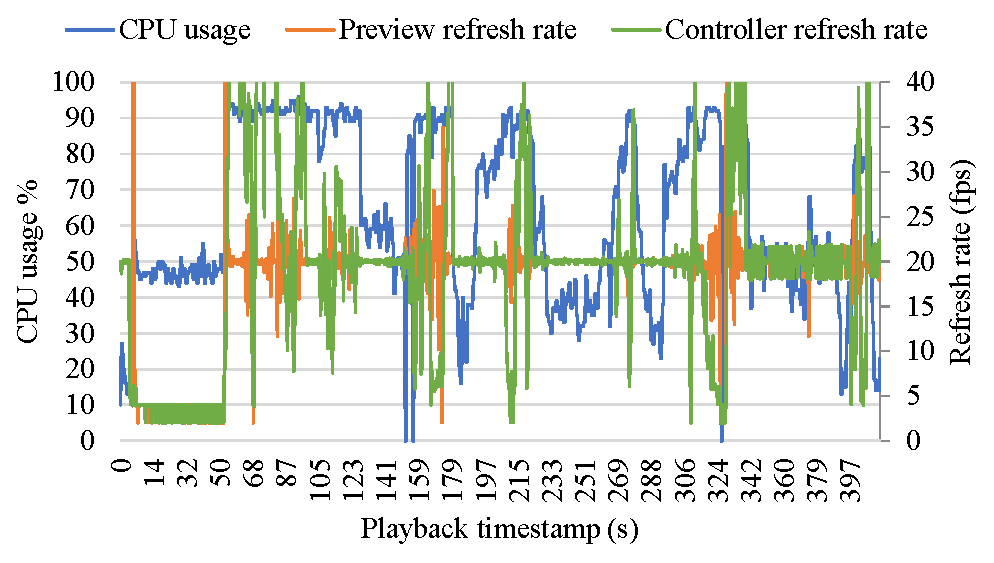
\includegraphics[width=0.8\columnwidth]{original}
    \caption{Performance of Vixen execution engine}
    \label{fig:original}
\end{figure}

Further analysis using Microsoft Visual Studio's sampling profiler shows, around $65 \%$ of CPU time was wasted between translation layers for generating controller commands, while the actual command assignment taking less than $1 \%$ of CPU time. There are several different command formats possible, for example 8-bit, 16-bit and RGB channels. Therefore, the application need to resolve the actual format of commands from their base type, which is apparently very inefficient in C\#. This process is called \texttt{dispatch} in the source code, it must be reduced or removed to improve performance. \wn{3}

The implementation of preview display was also inefficient, using around $20 \%$ CPU time in later stages.

\cmt{Different real-world sequence examples}

\subsection{Performance on Linux}

\cmt{Necessary GUI modification, imperfect GUI, tested with mono.}

\cmt{Insert screenshots...}

\section{Extract rendered sequence}

Instead of trying to improve the original execution engine, the performance problem may be eliminated by playing back stored data frames directly to individual hardware controllers. Thus, two steps are needed. Pre-rendering the sequence with accurate frame interval, then playback the rendered data to the controllers.

\subsection{Custom controller}

A custom controller module was developed based on one of its existing controllers. This controller uses TCP connection to transfer display data, supporting up to 65535 channels. A corresponding server application that simulates a multi-channel display was also developed using C++ and OpenGL \cite{shreiner2009opengl} rendering. Having this configuration allows debugging real-time display output without the need of a complex actual lighting controller setup. Data dumping, performance and statistical analysis can also be easily achieved. \wn{4}

The server application consumes less than $3 \%$ of CPU time under 50 fps refresh rate, which is negligible. It can also be executed on other computers, simulating real world network connection scenarios.

\subsection{Export sequence}

Although the custom controller module is capable of dumping outputs, it would not give the indication of sequence start and end information, and can have unstable frame rates influenced by CPU usage. Therefore, the sequence export function from sequence editor was used to dumping outputs.

The export function was originally used to convert the display sequence to formats recognisable by other applications and controllers. Most importantly, it renders the sequence using a manual timing source, gives accurate constant interval data dumps and controller channel mapping information. A customised data format was added to the export wizard, that can be later used for playback. \wn{5}

\cmt{Example XML file content?}

\cmt{Custom resolution modification?}

\cmt{Insert screenshots...}

\section{Controller specific implementations}

\cmt{Alternative baseline implementations for performance comparisons}

\subsection{Qt2 based on handheld device}

\cmt{Qt2 based, Noah NP1380, performance... \wn{10}}

\subsection{Minimal C\# implementation}

\cmt{VixenLinky, TCP data transfer \wn{11}}

\cmt{Performance on different hardware platforms \wn{12}}

\cmt{\texttt{BinaryReader} IO performance and buffer size \wn{14}}

\section{The new playback engine}

Based on the exported data format, an independent playback engine was developed and integrated into Vixen. \wn{6}

\cmt{The details of implementation, processing, performance critical steps skipped. \wn{6}}

\cmt{XML reading, serialiser}

\cmt{User interface..., does not support preview}

\cmt{Insert screenshots...}

\subsection{Performance and optimisations}

\cmt{Export performance and file sizes}

\cmt{Threading and mutex lock structure difference}

\cmt{Dictionary lookup replaced \wn{14}}

\fref{fig:playback} shows the performance of the playback engine. At the first and the last few seconds, the playback stopped, the system was using the original execution engine in idle. However, this engine still uses about $30 \%$ of CPU time. But, as soon as playback started, CPU usages drops to around $6 \%$ with stable refresh frame rates.

\begin{figure}[t]
    \centering
    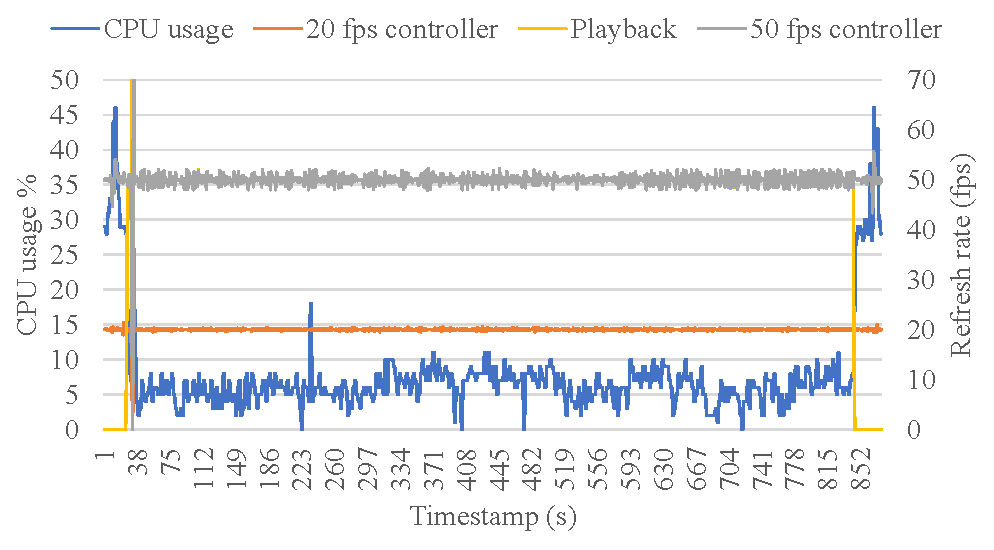
\includegraphics[width=0.8\columnwidth]{playback}
    \caption{Performance of new playback engine}
    \label{fig:playback}
\end{figure}

\subsection{Integration}

A separate menu entry was added to control the new playback engine. When the engine starts, it takes priority over the original execution engine.

\subsection{Audio playback}

The network configuration XML file generated from export was modified to include the audio media file used in the original sequence. This field was later used in the playback engine for audio playback, using the same audio functions from sequence playback. \wn{7}

\subsection{Scheduler integration}

The playback control was also integrated with built-in schedulers. It can therefore be scheduled to execute multiple times at specific time, possibly with original sequence schedules. \wn{8}

\cmt{Insert screenshots...}

The scheduler pre-process all scheduled items first. The sequences need to be pre-rendered, which can take a significant amount of time. The new playback engine does not need pre-process, can be directly executed within seconds.

\section{Console application}

\cmt{Implemented CUI version of Vixen. \wn{13}}

\subsection{Implementation}

\cmt{Uses original codebase (\texttt{Vixen.dll}), but only minimal initialisation and no GUI.

Loads modules from DLLs, especially controllers support.

Configuration modification? Modify XML directly, or program interfaces.}

\subsection{Loading performance}

\cmt{DLL module loading times...}

\cmt{Configuration file sizes... Tidy implemented}

\cmt{Profilers... \wn{14}}

\subsection{Execution performance}

\cmt{Slower than controller specific, analysis}

\cmt{Profilers...}

\subsection{Platform performance benchmark}

\cmt{Now possible with complete implementation on Linux}

\cmt{Unlimited playback and / or controller update speed for IO / processing comparison. \wn{15}}

\section{Video data format}

\subsection{Similarity}

\cmt{The whole process looks similar to animation designing, video rendering and playback}

\subsection{Implementation}

\cmt{Using ffmpeg for encoding and muxing in export, decoding and demuxing in playback}

\cmt{Using fmod for audio rendering to selectable devices}

\cmt{Using Interop for interfacing C/C++ DLLs to C\#. However, complex C/C++ data structure and processing require additional encapsulation in C/C++ \wn{17}

C/C++ and C\# implementation of basic encoding / decoding for testing.

Audio muxing and metadata for combining files. \wn{18}

\texttt{Makefile} and \texttt{diff} for automatic building and testing. \wn{17}}

\subsection{Benefits}

\cmt{Uses video to combine sequence dump, audio and configuration information into a single file, with reduced size \wn{16}}

\cmt{Easy sharing, editing software exists, sophisticated compress methods, hardware acceleration possible}

\subsection{Limitations}

\cmt{Small resolution for large number of channels, may not leverage full advantage of hardware video decoding}

\cmt{Discrete rapid-changing unassociated continuous channels not suitable for common video encoding methods and pixel formats:

Colour space, colour degrade, channel cross-talk}

\subsection{Integration}

\cmt{C\# interface, integrated directly to \texttt{Vixen.Sys} \wn{18}}

\cmt{Using newer version of fmod\wn{19}}

\cmt{Integrated to playback engine, switch based on file extension}

\subsection{Performance}

\cmt{Varies encoding, formats, quality factor... Insert data table \wn{16}}

\section{User Guide}

\cmt{\url{http://www.imperial.ac.uk/electrical-engineering/internal/current-students-course-handbook/msc-individual-research-project/writing-the-report-}}

\section{Conclusion}

\cmt{Varies methods of analysing and optimising resource intensive application. Now possible on an embedded platform for greater flexibility and power efficiency.}

\subsection{Limitations}

\cmt{Lower performance than controller dedicated applications

Video format not very useful for editing

Increased user interface complexity}

\subsection{Future works}

\subsubsection{Implementation improvements}
\hfill
The integration between original execution engine and the new playback engine can be improved. Currently, the playback engine takes priority over the execution engine, which might cause unwanted behaviour under certain circumstances. Playback contexts may also be implemented to cache multiple playback sequences information. The engines should be switched off during idle to further reduce CPU usage.

Support for preview display was not implemented for the playback engine, since the preview works in elements workspace whereas the playback engine works entirely in hardware controller workspace. It might be possible to extract mapping configurations during export, but support for preview is considered optional with lower priority.

\subsubsection{Video channel mapping}
\hfill
\cmt{Map channels as preview layout? For easy preview and modification using existing software.}

% references section
\bibliographystyle{IEEEtran}
\bibliography{Reference}

% that's all folks
\end{document}
